\chapter{Introduction}

Based on a rough estimate, there are about \num{10000} trillion ants, \num{7.6} billion humans, and a few million elephants in the world.
When considering this data set, one might come to the conclusion that there are more small objects in the world than there are large objects.
It so happens that this conclusion not only holds true on Earth, but it also holds true in our universe.
For every singular large object in space, there are significantly more smaller objects.
To provide a parallel to the animal example, in our solar system, there is one star, eight planets, and an almost incomprehensible number of small rocks traveling through space. 

In space, distances are presented on an extremely large scale when compared to on-Earth distances.  
Similarly objects in space travel significantly faster than objects observed on earth.
For example, the Earth travels at approximately \SI{30}{\kilo\meter\per\second} while small rocks can travel between \SIrange{11}{70}{\kilo\meter\per\second}.  
The speeds of these rocks exceed the muzzle velocity of a bullet \cite{russell_photometry_2018}.
When we observe a meteor shower, we are witnessing a barrage of these bullet-like rocks.  
Fortunately for mankind, Earth’s atmosphere provides a protective shield.
This shield is composed of tightly packed (relative to the vacuum of space) air molecules.

As a rocky object travels through Earth’s atmosphere, it collides with particles and burns in a phenomena known as ablation.  
The result is a release of energy in the form of both heat and light.  
The objects, which ignite and begin to break down are called meteors.
As a meteor releases light, the brightness can be measured from Earth's surface and is expressed as a photometric (visual) magnitude. 
The brightest meteors, which have a magnitude less than $-4$, are referred to as fireballs.
By observing the magnitude, duration, and other properties of individual fireball events, an observer can estimate impact energies and sizes of these near-Earth rocky objects.
Given a large enough sample size, observers can also determine the flux, or the number of events within a specific area per time, of fireballs of varying sizes and energies.

\begin{figure}[ht!]
  \centering
  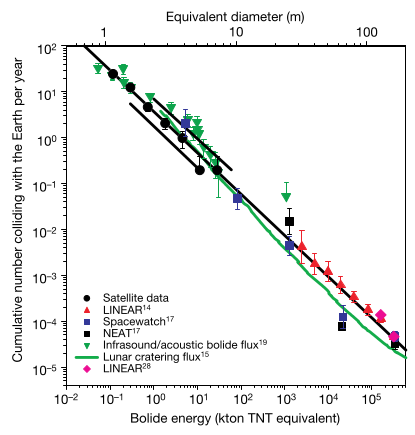
\includegraphics[scale=0.7]{images/flux_brown.png}
  \caption{A plot of bolide flux vs. energy and diameter using a wide collection of data}
  \label{brown}
\end{figure}


Flux can be calculated using any area, which is useful considering that an individual observer cannot monitor the entire earth's atmosphere.
In fact, any individual camera system can only observe up to around 0.03 percent of Earth’s total sky \cite{russell_photometry_2018}.
It follows that more camera systems located intentionally on earth's surface will give a more precise measurement of flux.  
While cameras set up by organizations such as NASA and the Spanish Meteor Network (SPMN) provide useful and precise measurements of fireball events, they lack flexibility and affordability.  
Often rendered immobile due to their connection to powerful computers, these systems are not nearly as versatile as the D6 Willamette AllSky survey. 

This project aims to analyze the feasibility of the Willamette D6 AllSky camera, a new alternative camera system for conducting fireball research. 
Occupying about the same space as a traffic cone, this camera is easily transportable and does not require an expensive computational base.
To determine the feasibility of our setup, we will compare our measured flux rates to those found by more well-recognized systems.
Peter Brown, an astronomy researcher, created a now-famous relationship between flux and bolide energy/diameter. 
As seen in Fig. \ref{brown}, bolides with extremely high energies are far less likely to collide with earth than their less powerful counterparts.
By comparing our flux rates to those found in Fig. \ref{brown} (for small energies), we can assess how consistent our data is with professional systems.

This paper is broken up into several sections for ease of reading. Chapter 2 details useful information surrounding fireballs, their importance, existing research, and the theory necessary to calculate flux rates.
